\section{Theory motivation}
\label{sec:theory}

\subsection{Landscape of theories proposing particle dark matter}
10,000 foot overview of theories that predict dark matter particles in this mass range. Note any interesting properties of the predicted particles, e.g., requires spin-dependent or EFT coupling, Can we say something about their preferred cross-section ranges in a finite number of plots?

\begin{figure}
    \centering
    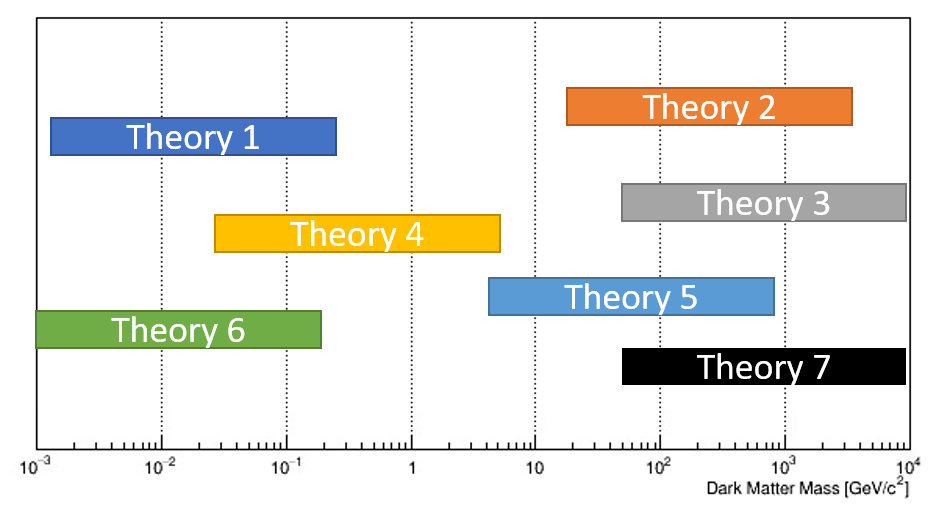
\includegraphics{figures/theory_landscape_cartoon.png}
    \caption{Range of WIMP masses predicted by various BSM theories. Y-axis has no meaning. Maybe use shape or shading to indicate preferred ranges}
    \label{fig:theor_wimp_masses}
\end{figure}

\begin{table}
    \centering
    \begin{tabular}{lcl}
    Theory name & Mass range & Notes \\ \hline
    Theory A & 1-1000 & \\
    Theory B & 0.01-10 &  only axial-vector couplings permited \\
    \end{tabular}
    \caption{Summary of theories predicting WIMPs}
    \label{tab:my_label}
\end{table}

\subsection{Complementary searches?}
Very short section on accelerator and atmospheric complementarity.